% Timing and presentation directions live in the separate storyboard.
\tikzset{
  sem early node/.style={
    draw=UITBlue!42!white, fill=UITBlue!6!white, rounded corners=2pt,
    minimum height=9mm, inner xsep=4mm, inner ysep=2mm, align=center
  },
  sem early destination/.style={
    sem early node, draw=UITBlue!82!black, fill=UITBlue!11!white
  },
  sem early arrow/.style={->, >=stealth, semithick, draw=UITBlue!82!black}
}

{\SemOpeningColors
\begin{frame}[t]
  \vspace*{3.5mm}
  \noindent
  \begin{minipage}[c]{17mm}
    {\setlength{\fboxsep}{2.3mm}\colorbox{white}{
\includegraphics[width=12mm]{assets/uit-emblem.png}}}
  \end{minipage}\hspace{3.8mm}%
  \begin{minipage}[c]{.80\linewidth}
    {\color{CoverMuted}\fontsize{8.7}{12}\selectfont ĐẠI HỌC QUỐC GIA TP. HỒ CHÍ MINH\par}
    {\SeminarSemibold\color{white}\fontsize{10.7}{15}\selectfont TRƯỜNG ĐẠI HỌC CÔNG NGHỆ THÔNG TIN\par}
  \end{minipage}\par

  \vspace{7mm}
  {\SeminarSemibold\color{Cyan}\fontsize{9.9}{13}\selectfont SEMINAR HỌC PHẦN\par}
  \vspace{2.3mm}
  {\SeminarHeavy\color{white}\fontsize{23}{28}\selectfont
    Deep Links và App Links\\trên Android\par}
  \vspace{2mm}
  {\color{CoverMuted}\fontsize{12.4}{16}\selectfont Một liên kết, hai đích đến\par}

  \vspace{4.5mm}
  {\color{UITBlue}\hrule width 20mm height .85pt}
  \vspace{2.9mm}
  {\color{white}\SeminarSemibold \SeminarCourse\par}
  {\color{CoverMuted}Giảng viên phụ trách · \SeminarLecturer\par}
  \ifdefempty{\SeminarTeam}{}{{\color{CoverMuted}Trình bày · \SeminarTeam\par}}
\end{frame}
}

\begin{frame}[t]{Vì sao một lần bấm mở đúng nội dung?}
  \SemLead{Bạn muốn xem lịch của một ngày cụ thể trên điện thoại.}
  \SemCols{%
    \SemCard{Bấm biểu tượng}{Mở ứng dụng, chuyển đến Lịch học, rồi chọn ngày.}%
  }{%
    \SemBlueCard{Bấm một dòng trên widget}{Mở Lịch học với ngày của buổi học đã được chọn.}%
  }
  \SemCallout{\textbf{Deep link} đưa người dùng tới một nội dung cụ thể trong ứng dụng. Ai chọn ứng dụng, và ai chọn nội dung?}
  \SemSource{\href{https://developer.android.com/training/app-links/}{Android Developers · About deep links}}
\end{frame}

\begin{frame}[t]{Tim Berners-Lee và bài toán tìm lại tài liệu}
  \SemLead{Ở CERN, thông tin kỹ thuật đã được ghi lại vẫn có thể khó tìm.}

  \noindent
  \begin{minipage}[t]{.35\linewidth}
    \vspace{0pt}
    \centering
    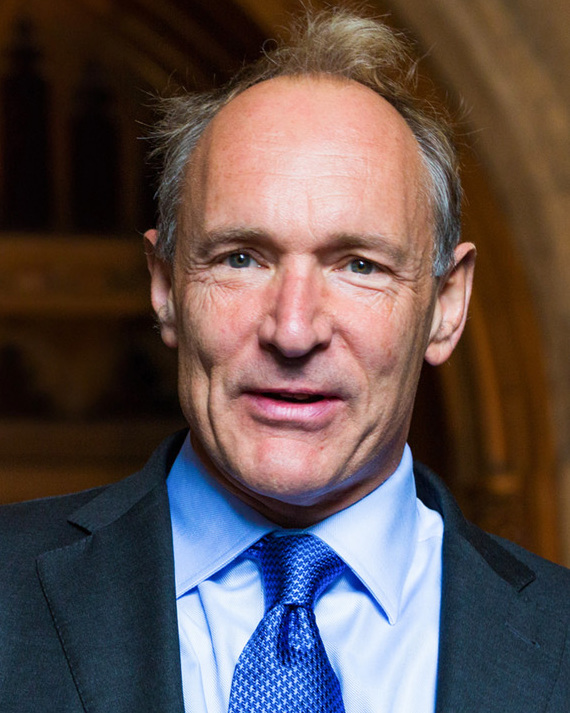
\includegraphics[height=37mm,width=\linewidth,keepaspectratio]{assets/history/tim-berners-lee-2014.jpg}\par
    \vspace{1mm}
    {\SeminarSemibold\small Tim Berners-Lee, 2014\par}
    {\scriptsize\color{Slate} Paul Clarke · cắt: KOKUYO\par}
    {\scriptsize\href{https://commons.wikimedia.org/wiki/File:Sir_Tim_Berners-Lee_(cropped).jpg}{Nguồn ảnh}
       · \href{https://creativecommons.org/licenses/by-sa/4.0/}{CC BY-SA 4.0}\par}
  \end{minipage}\hfill
  \begin{minipage}[t]{.61\linewidth}
    \vspace{0pt}
    \SemLabel{1989 · CERN}\par
    Tim Berners-Lee đề xuất dùng siêu văn bản để nối tài liệu, con người
    và dự án giữa nhiều nhóm và hệ máy.
    \par\medskip
    \SemLabel{1990 · WorldWideWeb}\par
    Berners-Lee và \mbox{Robert Cailliau} cùng viết đề xuất chính thức cho dự án.
    \par\medskip
    \SemCallout{\textit{“Often, the information has been recorded, it just cannot be found.”}\par
      {\scriptsize Đề xuất 1989}}
  \end{minipage}\par

  \SemSource{\href{https://www.w3.org/History/1989/proposal.html}{Đề xuất 1989} ·
    \href{https://www.w3.org/Proposal.html}{Đề xuất 1990} ·
    \href{https://home.cern/world-wide-web-35/}{CERN}}
\end{frame}

\begin{frame}[t]{Một địa chỉ dẫn sâu vào website}
  \SemLead{Tên host chỉ ra website. Path chỉ ra một trang bên trong website.}

  \noindent
  \begin{minipage}[t]{.455\linewidth}
    \vspace{0pt}
    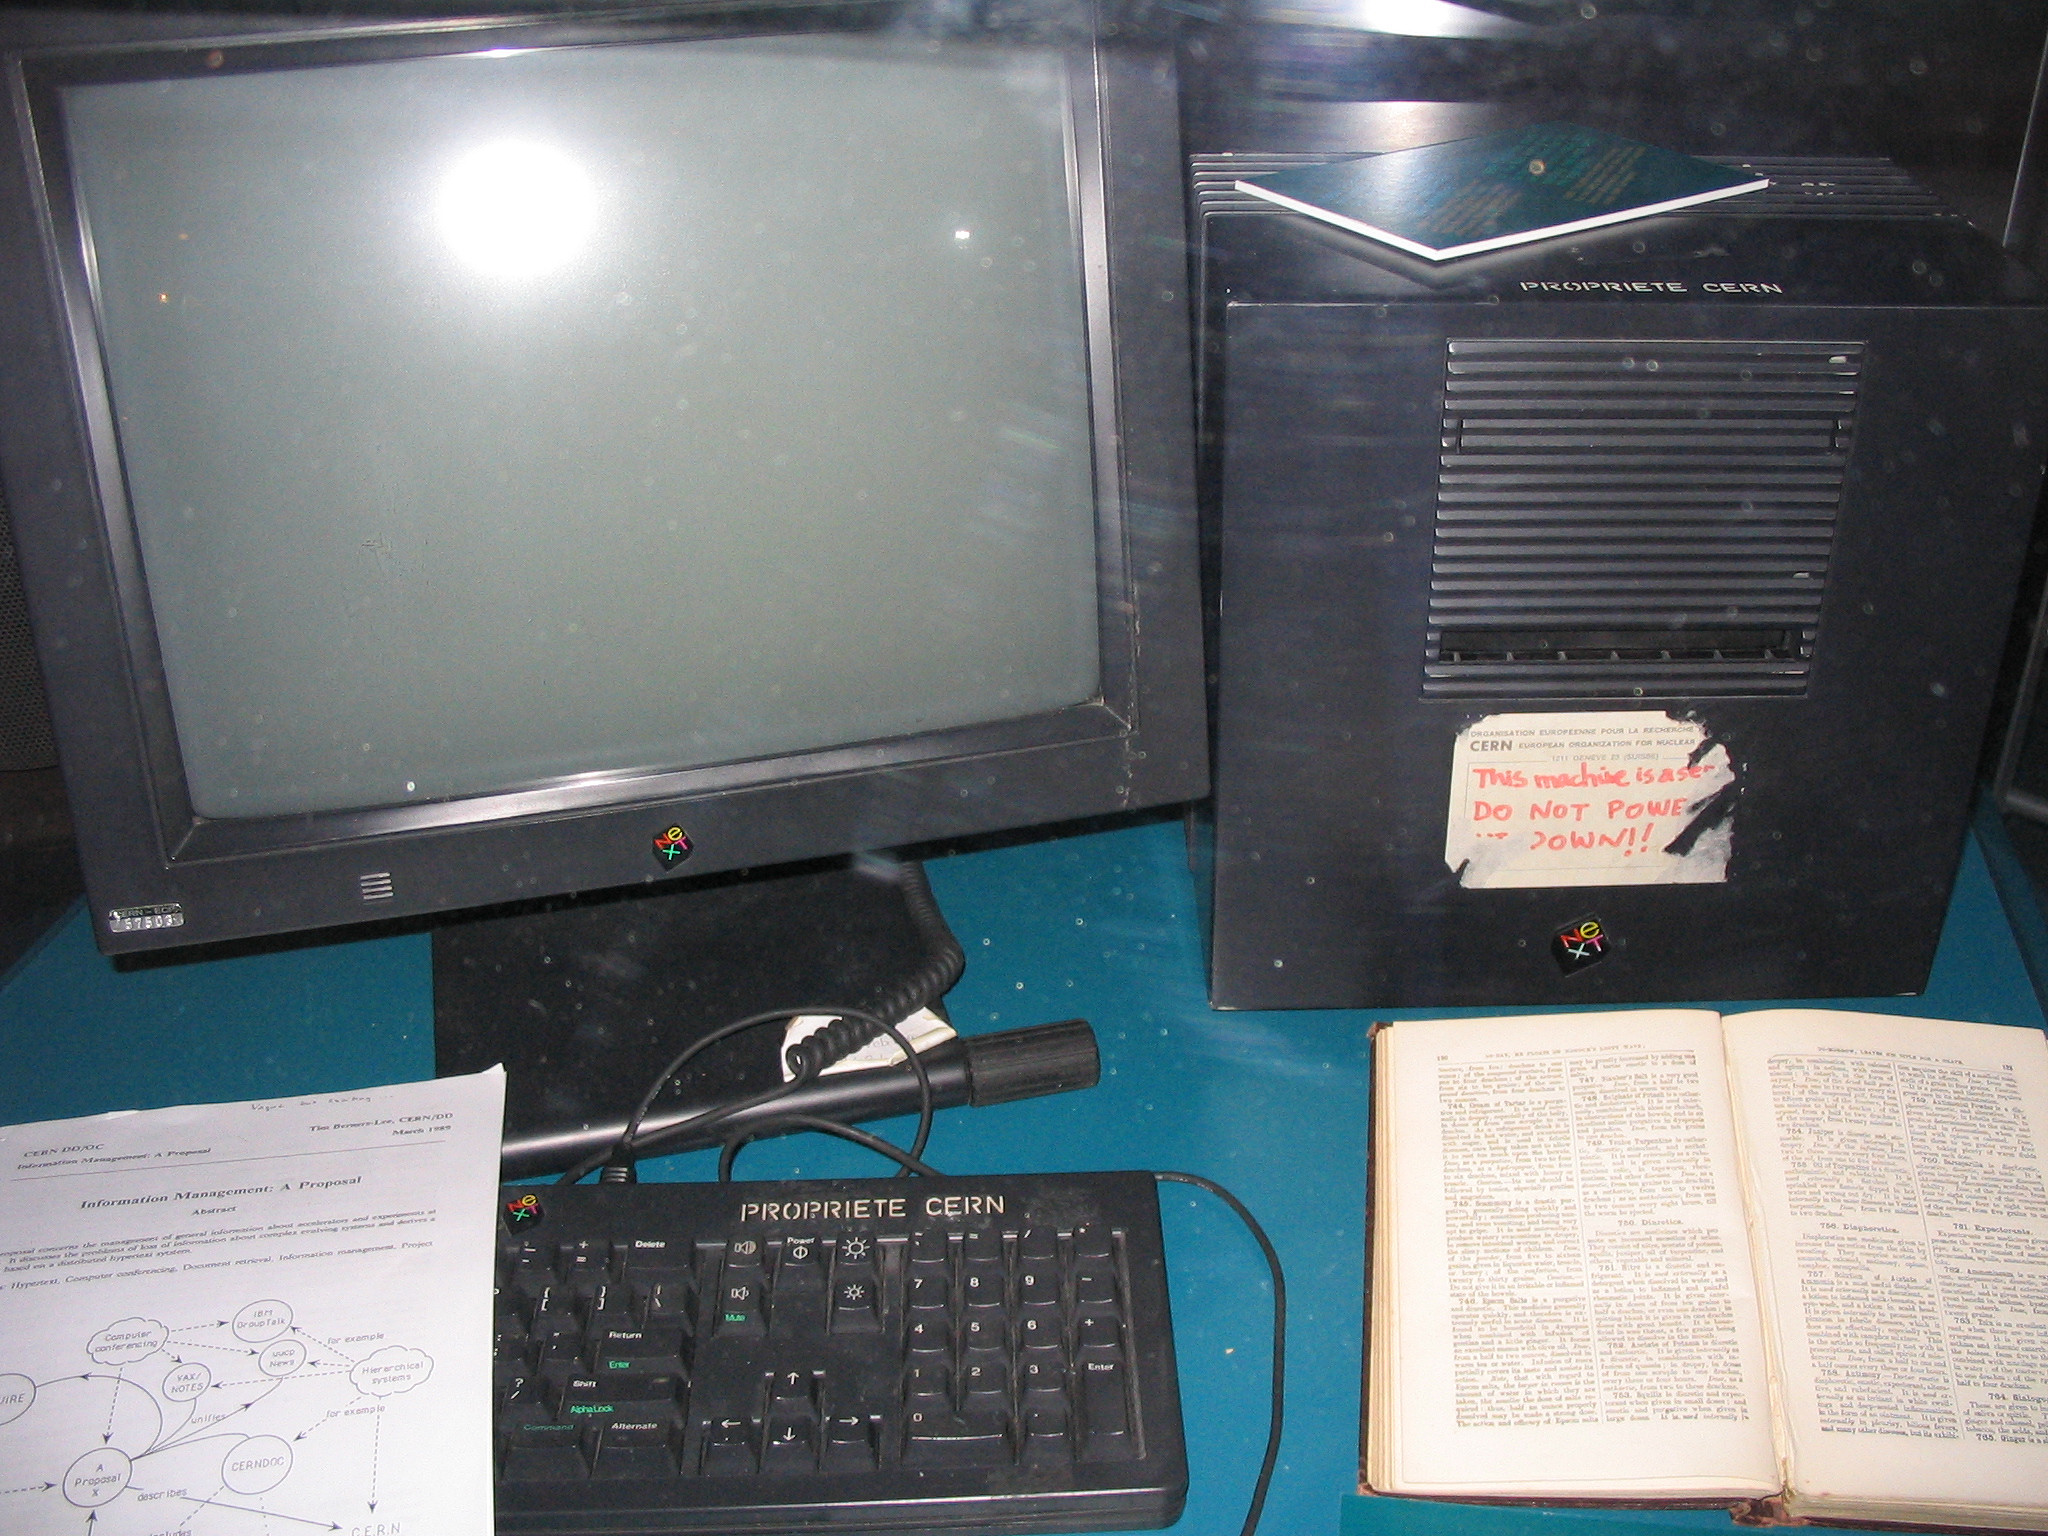
\includegraphics[width=\linewidth,height=34mm,keepaspectratio]{assets/history/first-web-server-cern-2005.jpg}\par
    {\SeminarSemibold\small Máy NeXT, máy chủ Web đầu tiên\par}
    {\scriptsize CERN, 2005 · \href{https://commons.wikimedia.org/wiki/File:First_Web_Server.jpg}{Coolcaesar}
      · \href{https://creativecommons.org/licenses/by-sa/3.0/}{CC BY-SA 3.0}\par}
  \end{minipage}\hfill
  \begin{minipage}[t]{.51\linewidth}
    \vspace{0pt}
    \SemCard{Địa chỉ trang World Wide Web}{%
      \href{https://info.cern.ch/hypertext/WWW/TheProject.html}{\texttt{info.cern.ch}}\par
      {\small\href{https://info.cern.ch/hypertext/WWW/TheProject.html}{\texttt{/hypertext/WWW/TheProject.html}}}%
    }
    \smallskip
    \SemLabel{1994 · RFC 1738}\par
    Đặc tả cú pháp URL.
    \par\smallskip
    \SemLabel{2003 · W3C TAG}\par
    \textit{Deep linking} trỏ tới trang bên trong website.
  \end{minipage}\par\smallskip

  {\small Một địa chỉ có thể lưu cả đích và bộ chọn nội dung, như đường tới lịch và ngày cần mở.\par}
  \SemSource{\href{https://home.cern/science/computing/the-birth-of-the-web/short-history-web}{CERN} ·
    \href{https://www.rfc-editor.org/rfc/rfc1738.html}{RFC 1738} ·
    \href{https://www.w3.org/2001/tag/doc/deeplinking-20030911}{W3C TAG, 2003}}
\end{frame}

\begin{frame}[t]{Android giao địa chỉ bằng Intent}
  \SemLead{Từ SDK Android 1.0 năm 2008, nền tảng đã có \SemCode{ACTION_VIEW}.}

  \noindent
  \begin{minipage}[t]{.65\linewidth}
    \vspace{0pt}
    \begin{tikzpicture}[
      stage/.style={sem early node,text width=14mm,inner xsep=2mm,minimum height=9mm},
    ]
      \node[stage] (sender) at (0,0) {\small App nguồn};
      \node[stage] (intent) at (2.3,0) {\small Intent};
      \node[stage] (android) at (4.6,0) {\small Android};
      \node[stage,fill=Ice,draw=Action] (receiver) at (6.9,0) {\small Activity};
      \draw[sem early arrow] (sender.east) -- (intent.west);
      \draw[sem early arrow] (intent.east) -- (android.west);
      \draw[sem early arrow] (android.east) -- (receiver.west);
    \end{tikzpicture}\par
    \smallskip
    \small\begin{tabularx}{\linewidth}{@{}L{.32\linewidth}Y@{}}
      \toprule
      \textbf{Yêu cầu} & \textbf{Thông tin mang theo} \\
      \midrule
      \SemCode{ACTION_VIEW} & Mở và hiển thị dữ liệu. \\
      URI & Địa chỉ, có thể mang ngày cần mở. \\
      Activity & Chỉ định đích hoặc để Android tìm. \\
      \bottomrule
    \end{tabularx}
  \end{minipage}\hfill
  \begin{minipage}[t]{.31\linewidth}
    \vspace{0pt}
    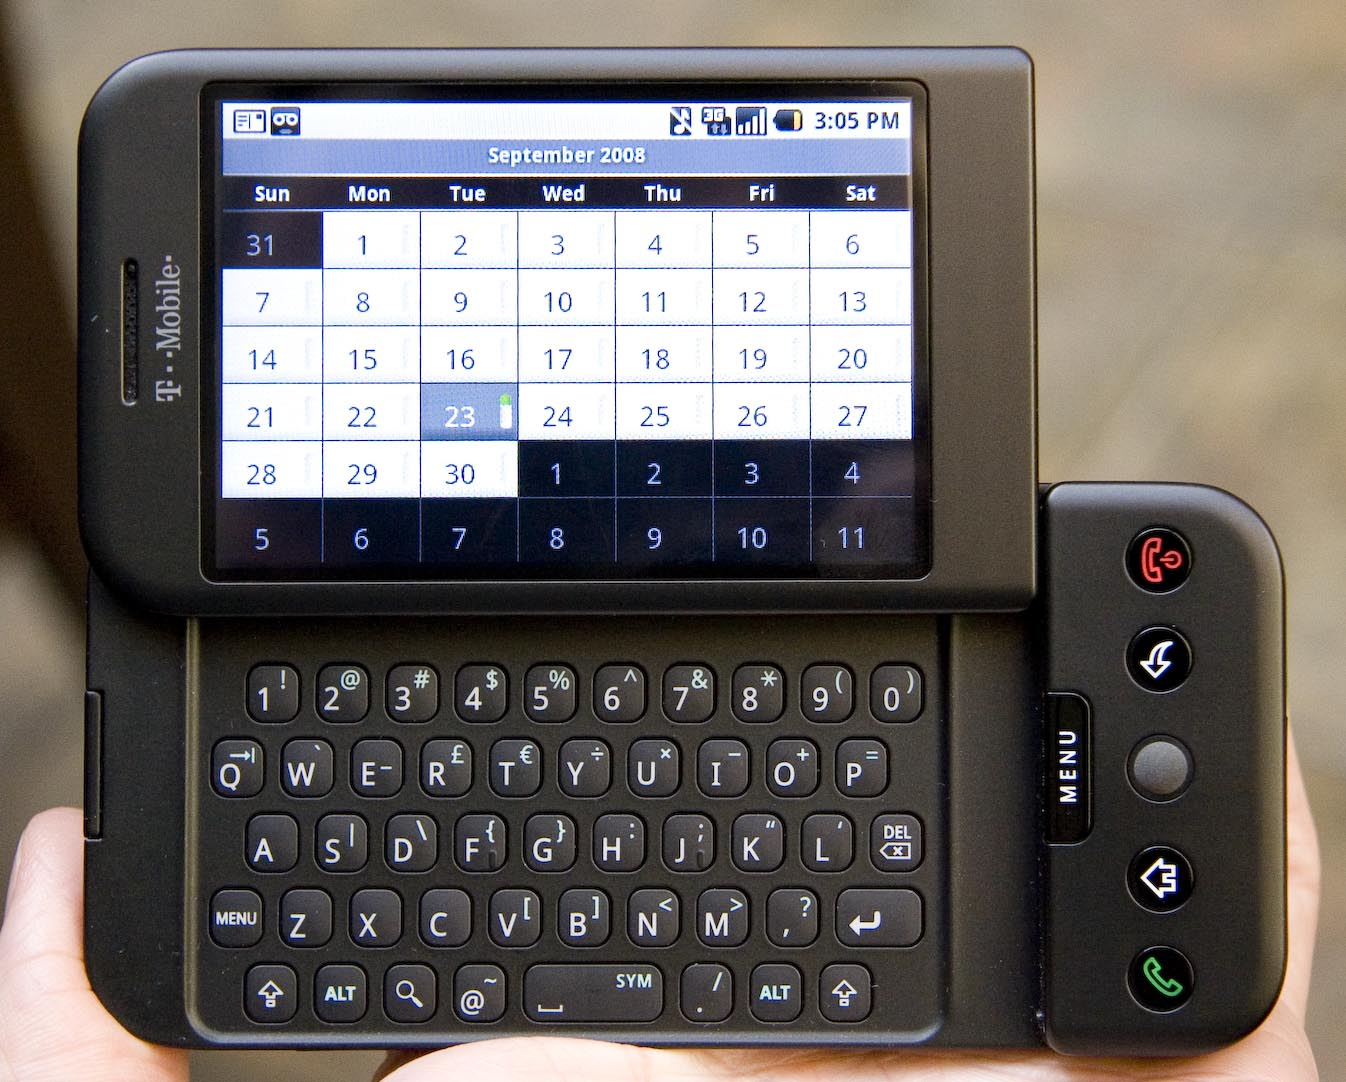
\includegraphics[width=\linewidth,height=27mm,keepaspectratio]{assets/history/tmobile-g1-launch-2008.jpg}\par
    {\SeminarSemibold\small T-Mobile G1, 2008\par}
    {\scriptsize\href{https://commons.wikimedia.org/wiki/File:T-Mobile_G1_launch_event_2.jpg}{Ảnh: Michael Oryl}
      · \href{https://creativecommons.org/licenses/by-sa/2.0/}{CC BY-SA 2.0}\par}
  \end{minipage}\par\smallskip

  \noindent{\small\textbf{2009 · OpenTable.} App khác mở thẳng luồng đặt bàn của một nhà hàng.\par}

  \SemSource{\href{https://android-developers.googleblog.com/2008/09/announcing-android-10-sdk-release-1.html}{Android 1.0 SDK} ·
    \href{https://developer.android.com/reference/android/content/Intent\#ACTION_VIEW}{ACTION\_VIEW} ·
    \href{https://android-developers.googleblog.com/2009/11/integrating-application-with-intents.html}{Ví dụ tích hợp năm 2009}}
\end{frame}

\begin{frame}[t]{Hai Activity có thể cùng nhận một URI}
  \SemLead{Với Intent ngầm định, Android tìm Activity có \textbf{intent filter} phù hợp.}

  \SemCols{%
    \begin{tabularx}{\linewidth}{@{}L{.36\linewidth}Y@{}}
      \toprule
      \textbf{Điều kiện} & \textbf{Ví dụ} \\
      \midrule
      Action & \SemCode{ACTION_VIEW} yêu cầu hiển thị. \\
      Category & Ngữ cảnh mở liên kết. \\
      Dữ liệu & Scheme, host và path xác định phạm vi URI. \\
      \bottomrule
    \end{tabularx}
  }{%
    \centering
    \begin{tikzpicture}[part/.style={sem early node,minimum width=18mm,inner xsep=2mm}]
      \node[part] (scheme) at (-2.17,0) {\small\SemCode{uit-mobile}\\[-.5mm]\scriptsize scheme};
      \node[part] (host) at (0,0) {\small\SemCode{widget}\\[-.5mm]\scriptsize host};
      \node[part] (path) at (2.17,0) {\small\SemCode{/schedule}\\[-.5mm]\scriptsize path};
      \node[sem early destination,minimum width=2.55cm] (a) at (-1.57,-1.68)
        {\textbf{Activity A}\\Khớp bộ lọc};
      \node[sem early destination,minimum width=2.55cm] (b) at (1.57,-1.68)
        {\textbf{Activity B}\\Khớp bộ lọc};
      \draw[sem early arrow] (host.south) -- ++(0,-.30) -| (a.north);
      \draw[sem early arrow] (host.south) -- ++(0,-.30) -| (b.north);
    \end{tikzpicture}\par
    {\small Giả sử cả hai đăng ký cùng URI.\par}%
  }

  \noindent Bộ lọc cho biết ai \textbf{có thể nhận}. Vậy ai được mở một URL công khai?\par
  \SemSource{\href{https://developer.android.com/guide/components/intents-filters}{Intents và intent filters} ·
    \href{https://developer.android.com/training/app-links/create-deeplinks}{Create deep links}}
\end{frame}

\begin{frame}[t]{Google Search mở nội dung trong app}
  \SemLead{31/10/2013 · Google thử nghiệm \textbf{App Indexing} trên kết quả Search.}

  \SemCols{%
    \centering
    \begin{tikzpicture}[early search card/.style={
      sem early node,minimum width=5.4cm,minimum height=7.5mm,inner ysep=1mm,
    }]
      \node[early search card] (search) at (0,0) {\textbf{Tìm phim Gravity}};
      \node[early search card] (result) at (0,-1.04) {Kết quả Rotten Tomatoes\\\textbf{Open in app}};
      \node[early search card,fill=Ice,draw=Action] (film) at (0,-2.08)
        {\textbf{Chi tiết phim trong Flixster}};
      \draw[sem early arrow] (search.south) -- (result.north);
      \draw[sem early arrow] (result.south) -- (film.north);
    \end{tikzpicture}\par
    {\small\href{https://3.bp.blogspot.com/-8TcQbpRIeC0/UnI7E47pp7I/AAAAAAAACtE/mf2PvzkLpqg/s1600/Flixster-app-indexing.png}{Hình gốc trong bài công bố, 2013}\par}%
  }{%
    \SemLabel{WEBSITE VÀ APP}\par
    Rotten Tomatoes khai báo trang phim tương ứng trong Flixster đã cài trên máy.
    \par\smallskip
    \SemLabel{MỘT VÍ DỤ KHÁC}\par
    Bài của Lawrence Chang minh họa tìm nhà ở Mountain View rồi mở Trulia.
  }

  \noindent Search đưa ra liên kết nội dung. Android xét nơi nhận liên kết.\par
  \SemSource{\href{https://android-developers.googleblog.com/2013/10/making-your-app-content-more-accessible.html}{Chaesang Jung, Android Developers} ·
    \href{https://developers.google.com/search/blog/2013/10/indexing-apps-just-like-websites}{Lawrence Chang, Google Search Central}}
\end{frame}
